\section{The \simpleAlgo Algorithm}

In general, the term \textit{flowset}~\cite{conf/sigcomm/YuanCM07} is used to describe the stream formed from an aggregation of flows.
In the context of this chapter we are interested only in flowsets that cover a full hierarchy.
Furthermore, it is very practical to assign counters to measure flowsets that cover a full hierarchy, using wild-cards matching techniques widely available in any traditional network gear and over the shelf SDN switches~\cite{OVS, OF1.5}.

\begin{figure}
	\centering
    \subfloat[The hierarchical flowset $f_3 \cup f_4\cup f_5\cup f_6$ can be measured by measuring $f_0$.]{
        \label{subfig:hierarchical_flowset}{
            \begin{tikzpicture}[->,>=stealth',level/.style={sibling distance = 3cm/#1,level distance = 1.5cm}]
            \coordinate (input);
            \node (a) [front, left=3cm of input] {$f_0$}
            child{ node [unexp] {$f_1$} 
                child{ node [unexp] {$f_3$}}
                child{ node [unexp] {$f_4$}}
            }
            child{ node [unexp] {$f_2$} 
                child{ node [unexp] {$f_5$}}
                child{ node [unexp] {$f_6$}}
            };
            \end{tikzpicture}
        }}
    \subfloat[The non Hierarchical flowset $f_3 \cup f_4 \cup f_6$, requires at least measuring $f_1$ and $f_6$.] {
        \label{subfig:HHH_second_epoch}{
            \begin{tikzpicture}[->,>=stealth',level/.style={sibling distance = 3cm/#1,level distance = 1.5cm}]
            \coordinate (input);
            \node (a) [non_front, left=3cm of input] {$f_0$}
            child{ node [front] {$f_1$} 
                child{ node [unexp] {$f_3$}}
                child{ node [unexp] {$f_4$}}
            }
            child{ node [non_front] {$f_2$} 
                child{ node [unexp] {$f_5$}}
                child{ node [front] {$f_6$}}
            };
            \end{tikzpicture}
        }
    }
\caption[An example of hierarchical flowsets and non hierarchical flowsets]{Example of hierarchical flowsets and non hierarchical flowsets, for the hierarchy covered by $f_0=39.128.128.128/30$.}
\label{fig:flowsets}
\end{figure}

The main concept of this algorithm and our general approach is to facilitate the widely available easy measuring of such flowsets to calculate a set of suspect Heavy Hitter Flows and Hierarchical Heavy Hitter Flows. These sets are created by following paths of suspect heavy hitters flowsets down a \textit{prefix trie}, where in each step the suspect flowset is broken into several disjoint flowsets to be measured independently. This follows the steps of~\cite{conf/sigcomm/YuanCM07,Moraney2016}.

In all of our algorithms, we identify each flow by a unique \textit{string} over some alphabet and each flowset by a regular expression over the same alphabet, such that all flows contained in the flowset are the flows represented by the strings matching the flowset's regular expression. The motivation behind this approach is to identify each flow by an IP address and each flowset by a CIDR mask, such that a flowset is the group of all flows that their corresponding binary representation of the IP address is included in the flowset's CIDR mask.

This definition also allows tracking multidimensional flows (e.g., pairs of $<$IP\_SRC,IP\_DST$>$) by extending the string representing the flow to 64 bits consisted from contacting both strings of the IP source address and IP destination address. Also, one might consider five tuple flows $<$IP\_SRC,IP\_DST,SRC\_PORT,DST\_PORT,PROTOCOL$>$ by contacting the binary strings of these fields from the IP header.

A main property of our general approach is that we limit the number of counters used by the algorithms a priori. That is, the number of counter available for monitoring is given as input (we usually use $C$ to indicate this number see Table \ref{tab:def}) and the monitoring algorithm can not use  more than this number of counters.
With this limitation in hand, the main observation that motivates the algorithm, is that each HH flow in any level of the hierarchy mandates a HH flow in the upper levels of the hierarchy up to the root.

We note that given a threshold $\phi$ there can be no more than $\floor{\frac{1}{\phi}}$ HH in a given level and no more than $\floor{\frac{1}{\phi}}$ HHH in all the levels together.
Furthermore, a HHH flow in a given level must be a HH flow in that level since the conditional frequency of the a flowset is at most its frequency.
Thus, the algorithm tries to zoom in on HH flows by splitting the flowsets for which the overall traffic is greater than the threshold down to the lower level of the hierarchy. After detecting the suspect HH in all of the levels, the algorithm builds in a bottom-up approach the set of suspect HHH by calculating their conditional frequency.

A critical aspect of the algorithm is deciding when to investigate further the suspect flowsets, i.e., when to split the flowsets. Given the length of trace, the number of counters ($C$) and the depth of the hierarchy ($H$), the algorithm partitions the trace into $H+1-log_2(C)$ parts and performs a round of monitoring for each part. These parts, unless specifically stated, are usually equal. It is possible to partition the trace either by number of packets, by byte count or by time. Partitioning the trace by time is the most straightforward approach and only requires knowing the length of the monitoring period and could be user specific.

For each packet the algorithm updates exactly one counter, however, the algorithm performs $H+1-log_2(C)$ ``heavy" steps, at the end of each round. In these steps the algorithm decides which of the currently monitored flowsets to split into two smaller flowsets. Such step requires $O(C)$ operations and happens $O(H)$ times regardless of the number of packets. Thus, the algorithm has a constant per-packet operation.

The static nature of the splitting and the observations about the nature of HH and HHH flows in the hierarchy form the base for the \simpleAlgo Algorithm. The algorithm receives as input the number of counters, the depth of the hierarchy, the monitoring period and the threshold. As an initialization step, the algorithm partitions the hierarchy into $C$ flowsets and allocates a counter per each flowset. This means that the algorithm assigns a counter for each flowset in the level $log_2(C)$ of the hierarchy, as shown in figure~\ref{fig:init}.

\begin{figure}
	\centering
    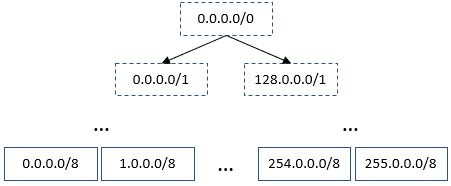
\includegraphics[width=\linewidth]{HHH/jpg_figures/init.JPG}
\caption[An example of partitioning the hierarchy given $256$ counters]{Given $C=256$ counters, the algorithm partitions the IP\_SRC hierarchy ($H=32$) at level $8$ into disjoint sets and assigns a counter per flowset.}
\label{fig:init}
\end{figure}

During each round, where packets with respective values arrive, their keys are extracted and the counter of the matching flowset is updated with the respective value. The keys of the packets depend on the flow definition the user is using, usually a single dimension of the IP addresses.
Furthermore, the respective values depends on which version of the problem we are tackling, the unweighted or the weighted version. In the unweighted version, we count the number of packets per flow, thus the values attached to each packets are 1. In the weighted version, we count the byte count of each flow, thus the values are the byte count field of the IP header.

At the end of each round, the algorithm takes decision regarding splitting flows. This means that the algorithm exams the aggregate values of the monitored flowsets and now should  filter out ``uninteresting" flowsets to allow allocating counters to finer (more specific) flowsets in order to move down the hierarchy. The most obvious candidates to refine are flowsets that had more than $\phi$ of the total frequency of the current period. However, since we refining each single flowsets into two flowsets, we have enough counter to refine the top $\frac{C}{2}$ flowsets. Thus, the algorithm sorts the monitored flowsets according to their counters values, refines the top $\frac{C}{2}$ and reassign the $C$ counter to monitor these new flowsets.

This refinement step happens $H-log_2(C)$ times, until the algorithm reaches that last level of the hierarchy. Then, a bottom-up process takes place to calculate the set of candidate hierarchical heavy hitters. This process is straightforward calculation of the conditional frequency of each previously monitored flowset and output those that exceed the threshold.

This calculation does not require any estimation of the frequencies between the rounds since the rounds are equal. This approach works extremely well if the streams are stable over time.  However,  fluctuations in the flow's frequencies among the rounds, might cause missing some of the HH and thus some of the HHH flows. This is, of course, the main drawback of the \simpleAlgo Algorithm.

One approach to tackle this drawback is splitting the trace into a smaller constant number of rounds (e.g. 4). This assumes, that the longer each round the more stable is the flows distribution among these rounds. This is the motivation behind the Multiple Split Algorithm presented below.

Another drawback of this algorithm is the lack of a ``reconsidering" mechanism. That is, if the algorithm does not split a given flowset in an early round it will never reconsider it, even if there is some flow in this flowsets that became later responsible for a large amount of the traffic in the trace.

\begin{algorithm}\small
    \SetKwInOut{Input}{Input}
    \SetKwInOut{Output}{Output}
    \Input{A stream of packets $S$, a threshold $\phi$, number of counters $C$ and the depth of the hierarchy $H$}
    \Output{set of hh and hhh in $S$}
    $F = init\_flowsets(C)$\;
    $number\_rounds=H+1-log_2(C)$\;
    \ForEach{$r$ in $\{1..number\_rounds\}$}
    {
        $counters=assign\_counters(F)$\;
        $packets=get\_round\_packets(r, number\_of\_rounds)$\;
        \ForEach{$counter$ in $counters$}{
            counter\_packets=$\{p\in packets : flow(p)\in counter.flow\}$\;
            counter.value=$\sum\limits_{p \in counter\_packets}value(p)$\;
        }
        \If{$r < number\_rounds$}
        {
            $top\_flowsets=sort(F, counters)[1:\frac{C}{2}]$\;
            $F=refine\_flowsets(top\_flowsets,1)$\;
        }
    }
    $hh\_per\_level=calculate\_hh\_per\_level(\phi)$\;
    $hhh\_per\_level=calculate\_hhh\_per\_level(\phi, hh\_per\_level)$\;
    return $hh\_per\_level, hhh\_per\_level$
    \SetAlgoRefName{\simpleAlgo}
    \caption{}
    \label{algo:simple_split}
\end{algorithm}
